\documentclass{standalone}
\usepackage{tikz}
\begin{document}

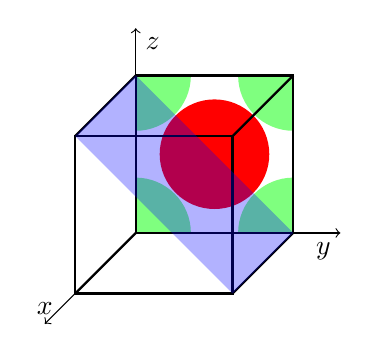
\begin{tikzpicture}[scale=2]
    \fill[green, opacity=0.5,] (0,0,0) -- (0.35,0,0) arc[start angle=0, end angle=90, radius=10pt] -- cycle;
    \fill[green, opacity=0.5,] (1,0,0) -- (1-0.35,0,0) arc[start angle=180, end angle=90, radius=10pt] -- cycle;
    \fill[green, opacity=0.5,] (1,1,0) -- (1-0.35,1,0) arc[start angle=180, end angle=270, radius=10pt] -- cycle;  
    \fill[green, opacity=0.5,] (0,1,0) -- (0.35,1,0) arc[start angle=360, end angle=270, radius=10pt] -- cycle;
    \node[circle, fill=red, inner sep=14pt] at (0.5,0.5,0) {}; % Atom at (0.5,0.5,0)

    \draw[thick] (0,0,0) -- (1,0,0) -- (1,1,0) -- (0,1,0) -- cycle; % Bottom face
    \draw[thick] (0,0,0) -- (0,0,1); % Vertical edge back-left
    \draw[thick] (0,0,1) -- (1,0,1) -- (1,1,1) -- (0,1,1) -- cycle; % Top face
    \draw[thick] (1,0,0) -- (1,0,1); % Vertical edge front-right
    \draw[thick] (1,1,0) -- (1,1,1); % Vertical edge back-right
    \draw[thick] (0,1,0) -- (0,1,1); % Vertical edge front-left
    
    % Label the axes
    \draw[->] (0,0,0) -- (1.3,0,0) node[anchor=north east]{$y$};
    \draw[->] (0,0,0) -- (0,1.3,0) node[anchor=north west]{$z$};
    \draw[->] (0,0,0) -- (0,0,1.5) node[anchor=south]{$x$};
    
    % Shading the (110) plane
     \fill[blue, opacity=0.3] (1,0,0) -- (0,1,0) -- (0,1,1) -- (1,0,1) -- cycle;
\end{tikzpicture}
\end{document}